\documentclass{article}

\usepackage{pgf}
\usepackage{tikz}
\usetikzlibrary{arrows,automata}
\usepackage[latin1]{inputenc}
\begin{document}
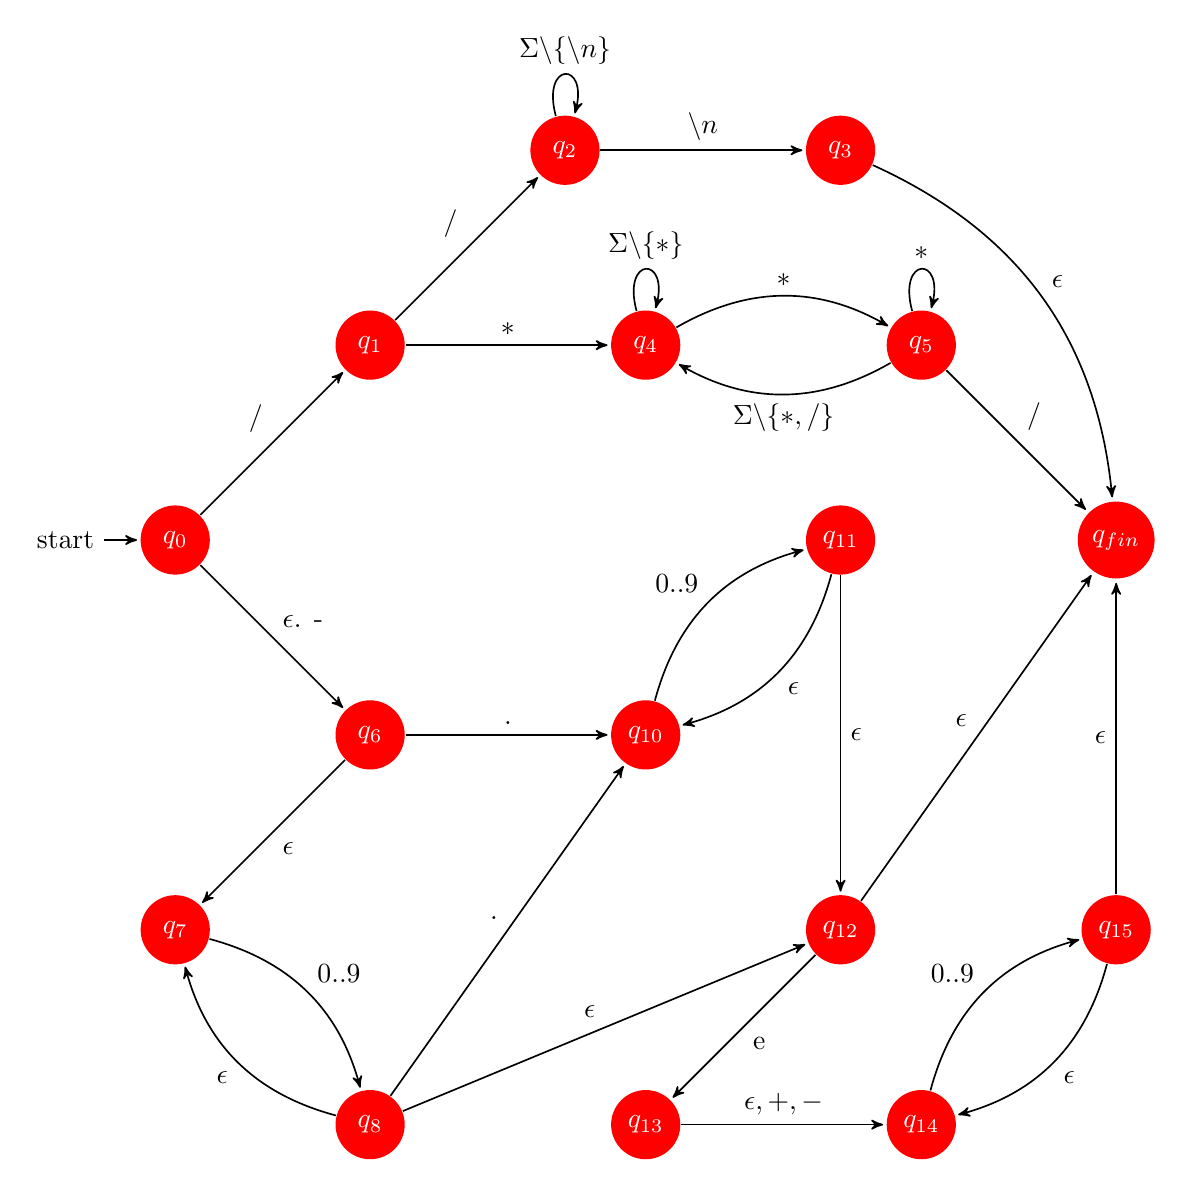
\begin{tikzpicture}[->,>=stealth',shorten >=1pt,auto,node distance=3.5cm,
                    semithick]
  \tikzstyle{every state}=[fill=red,draw=none,text=white]

  \node[initial,state]  (q0)                     {$q_0$};
  \node[state]          (q1) [above right of=q0] {$q_1$};
  \node[state]          (q2) [above right of=q1] {$q_2$};
  \node[state]          (q3) [right       of=q2] {$q_3$};
  \node[state]          (q4) [right       of=q1] {$q_4$};
  \node[state]          (q5) [right       of=q4] {$q_5$};
  \node[state]          (q6) [below right of=q0] {$q_6$};
  \node[state]          (q7) [below left  of=q6] {$q_7$};
  \node[state]          (q8) [below right of=q7] {$q_8$};
  \node[state]          (q10)[      right of=q6] {$q_{10}$};
  \node[state]          (q11)[above right of=q10]{$q_{11}$};
  \node[state]          (q12)[below right of=q10] {$q_{12}$};
  \node[state]          (q13)[below left  of=q12]{$q_{13}$};
  \node[state]          (q14)[right       of=q13]{$q_{14}$};
  \node[state]          (q15)[right       of=q12]{$q_{15}$};
  \node[accepting,state](qf) [right       of=q11] {$q_{fin}$};

  \path (q0) edge              node {$/$}        (q1)
             edge              node {$\epsilon$. -} (q6)
        (q1) edge              node {$/$}        (q2)
             edge              node {$*$}        (q4)
        (q2) edge [loop above] node {$\Sigma \symbol{92} \{ \symbol{92} n\}$} (q2)
             edge              node {$\symbol{92} n$} (q3)
        (q3) edge [bend left]  node {$\epsilon$} (qf)
        (q4) edge [bend left]  node {$*$}        (q5)
             edge [loop above] node {$\Sigma \symbol{92} \{*\}$}  (q4)
        (q5) edge              node {$/$}        (qf)
             edge [loop above] node {$*$}        (q5)
             edge [bend left]  node {$\Sigma \symbol{92} \{*,/\}$} (q4)

        (q6) edge              node {$\epsilon$} (q7)
             edge              node {.} (q10)
        (q7) edge [bend left]  node {0..9}       (q8)
        (q8) edge [bend left]  node {$\epsilon$} (q7)
             edge              node {.} (q10)
             edge              node {$\epsilon$} (q12)
        (q10)edge [bend left]  node {0..9}       (q11)
        (q11)edge [bend left]  node {$\epsilon$} (q10)
             edge              node {$\epsilon$} (q12)
        (q12)edge              node {$\epsilon$} (qf)
             edge              node {e}          (q13)
        (q13)edge              node {$\epsilon,+,-$}  (q14)
        (q14)edge [bend left]  node {0..9}       (q15)
        (q15)edge [bend left]  node {$\epsilon$} (q14)
             edge              node {$\epsilon$} (qf)
;

\end{tikzpicture}

\end{document}
